\chapter{Portraits de phases de systèmes non-linéaires}
    \section{Introduction}
    \section{Systèmes non-linéaires d'ordre 2}
        Soit un système dynamique non-linéaire défini par le système d'équations différentielles :
        \begin{equation}
            \begin{cases}
                \dot{x}_1 = f_1(x_1, x_2) \\
                \dot{x}_2 = f_2(x_1, x_2)
            \end{cases}
        \end{equation}
        où au moins une des fonctions $f_1$ ou $f_2$ est non linéaire. Dans le cas de systèmes non linéaires, l'analyse directe peut être complexe, voire impossible. Cependant, une approche standard pour comprendre le comportement local du système autour d'un point d'équilibre consiste à linéariser le système. Cette méthode s'appuie sur le développement de la fonction au voisinage de points spécifiques (typiquement des points d'équilibre) et permet d'extraire des informations cruciales sur la dynamique locale.

        Pour réaliser cette approximation linéaire \robin{dans le cas où $f_1$ et $f_2$ sont dérivables}, nous calculons la \textit{matrice jacobienne} du système, qui décrit la variation infinitésimale des fonctions $f_1$ et $f_2$ par rapport aux variables $x_1$ et $x_2$. La matrice jacobienne s'exprime comme suit :

        \begin{definition}{Matrice jacobienne}
            La matrice jacobienne d'un système est définie comme la matrice des dérivées partielles selon les composantes. Dans le cas d'ordre 2,
            \begin{equation}
                J = 
                \begin{bmatrix}
                    \pd {f_1}{x_1} & \pd {f_1}{x_2} \\
                    \pd {f_2}{x_1} & \pd {f_2}{x_2}
                \end{bmatrix}
            \end{equation}
        \end{definition}
        L'évaluation de cette matrice au point d'équilibre (en posant $\dot{x}_1 = \dot{x}_2 = 0$) fournit un système linéarisé, dont le comportement global autour de l'équilibre peut être interprété en analysant les valeurs propres de $J$.

        Les valeurs propres de cette matrice jacobienne jouent un rôle crucial dans la classification locale du point d'équilibre en tant que nœud, foyer, point-selle, ou centre :
        \begin{itemize}
            \item si les valeurs propres sont réelles et de même signe, le point d'équilibre est un nœud attractif ou répulsif~;
            \item si les valeurs propres sont réelles et de signes opposés, le point d'équilibre est un point-selle, indiquant un comportement divergent sur certaines directions et convergent sur d'autres~;
            \item si les valeurs propres sont complexes conjuguées avec une partie réelle non nulle, le point est un foyer, décrivant un comportement oscillatoire autour de l'équilibre~;
            \item si les valeurs propres sont purement imaginaires, le point d'équilibre est un centre, et le système suit des trajectoires fermées autour de ce point.
        \end{itemize}
        Notons que cette classification est uniquement valide si les valeurs propres de $J$ sont toutes deux non nulles, assurant que le point d'équilibre est non dégénéré.
        
    \section{Exercices}
        L’objectif est de mener une analyse complète de ces systèmes en plusieurs étapes, qui sont détaillées ci-dessous. Cette analyse permettra d’examiner la dynamique des solutions dans le plan de phase et d’approfondir notre compréhension des comportements locaux autour des points d'équilibre.
    
        \begin{enumerate}
            \item Calcul et tracé des isoclines.
            \item Détermination des points d'équilibre
            \item Calcul de la matrice jacobienne. Le calcul de $J$ pour chacun des systèmes aux points d’équilibre permet d'obtenir une approximation linéaire du comportement du système autour de ces points.
            \item Étude du comportement local avec la matrice jacobienne: au voisinage de chaque point d’équilibre, nous utilisons la matrice jacobienne pour analyser la stabilité locale, comme vu durant ce chapitre. En examinant les valeurs propres de cette matrice, nous déterminons la nature du point d'équilibre (nœud, foyer, point-selle, etc.) et décrivons le comportement local des trajectoires.
            \item Dessin du portrait de phase
        
        \end{enumerate}
        Cette démarche permet une compréhension approfondie de chaque système dynamique, tant au niveau local qu’au niveau global, en combinant linéarisation locale et analyse graphique pour obtenir une interprétation complète des trajectoires et des comportements des solutions.

        \subsection{Exercice 1}
            \begin{exercise}{Exercice 1}
                \begin{equation}
                    \begin{cases}
                        \dot{x}_1 = x_1 \\
                        \dot{x}_2 = x_1^2 + x_2^2 - 1
                    \end{cases}
                \end{equation}
            \end{exercise}
            La solution numérique est donnée à titre indicatif dans la figure \ref{fig:pdp_exercice_3_1}.
            \begin{figure}[ht!]
                \centering
                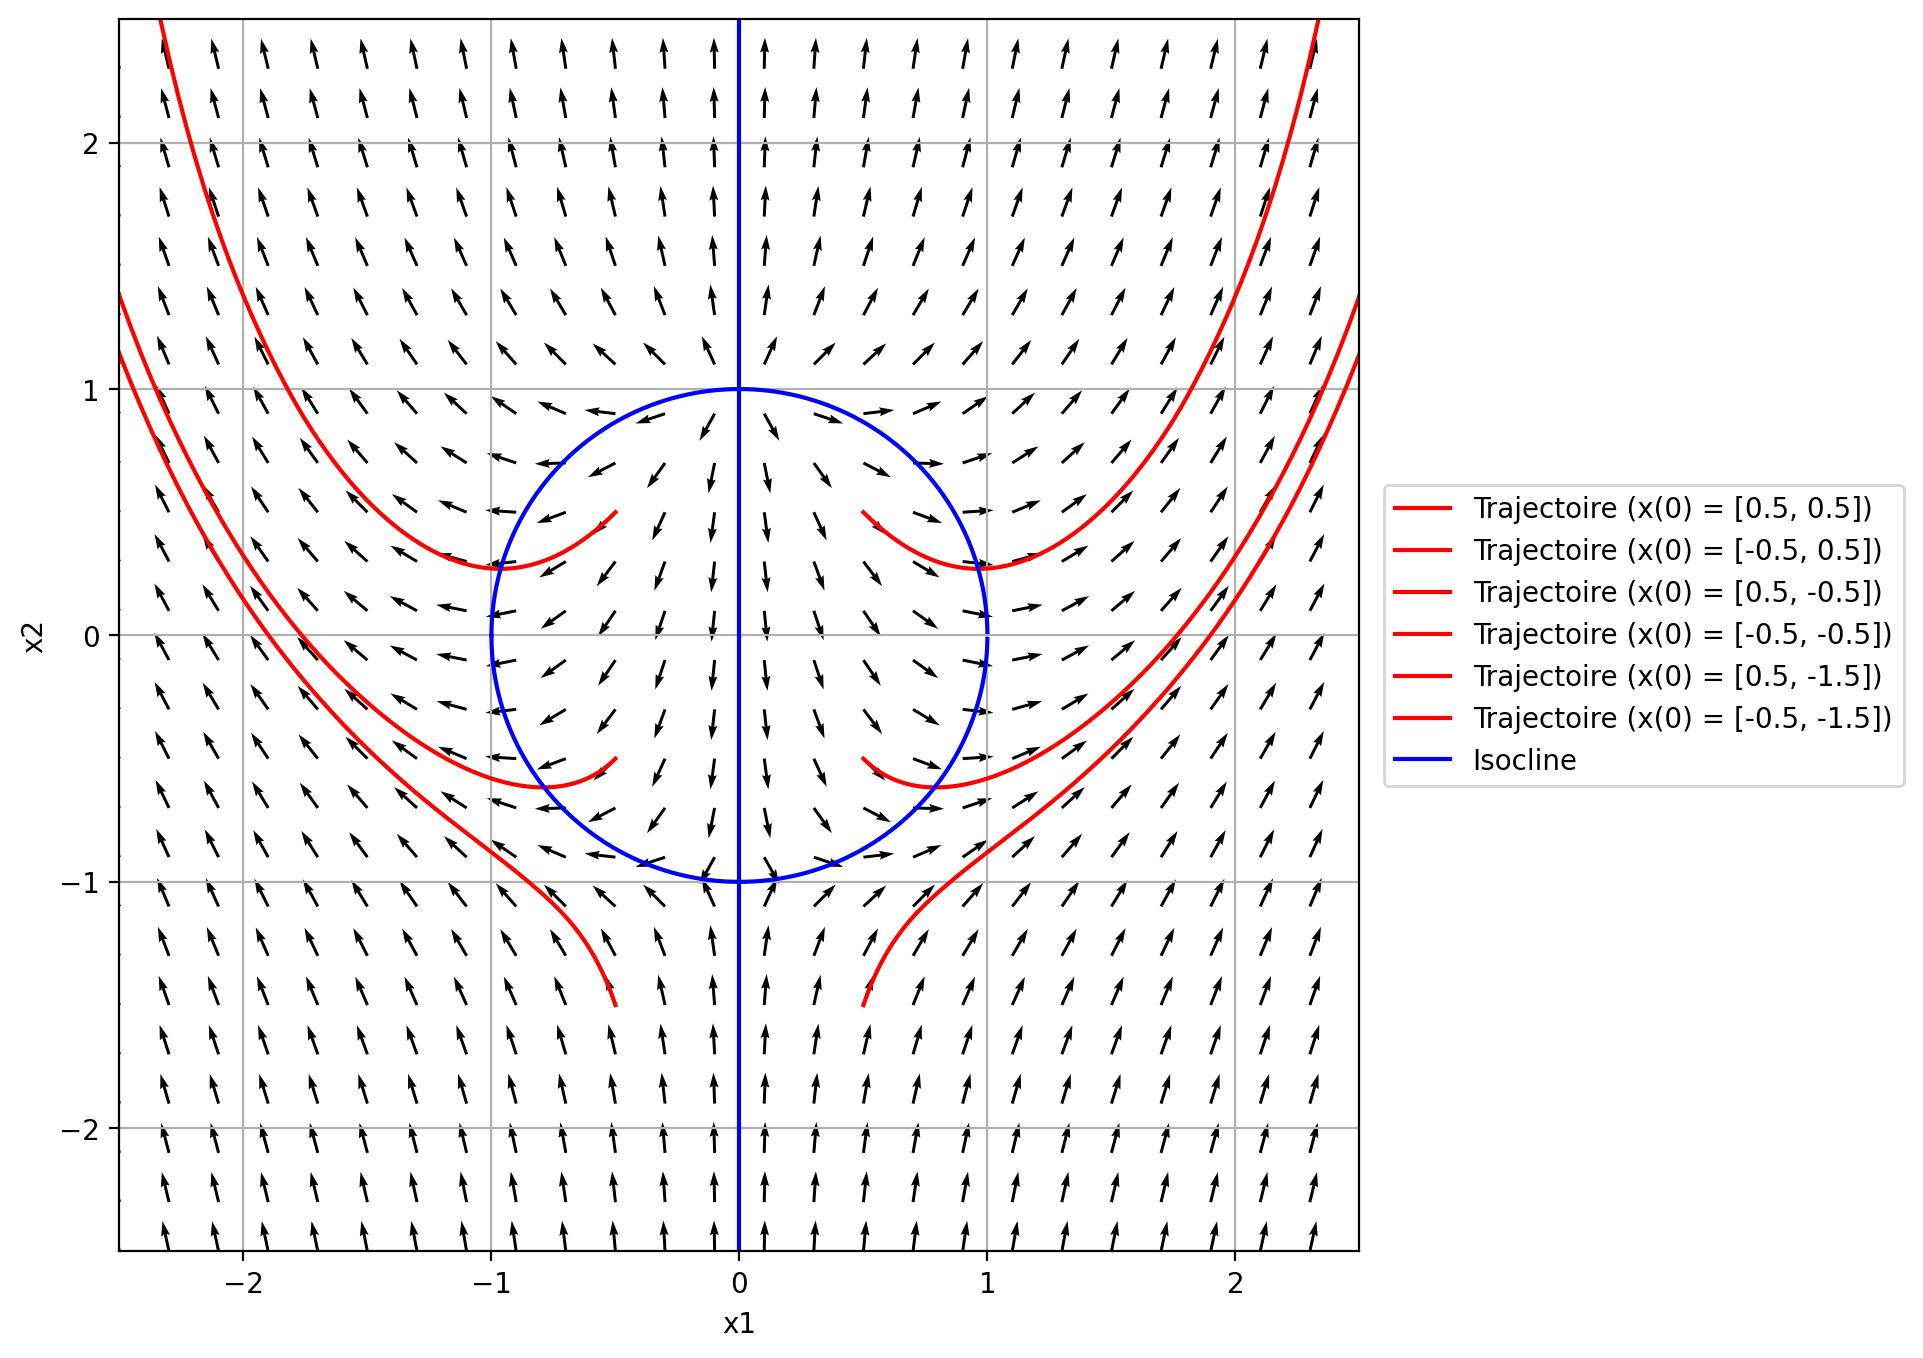
\includegraphics[width=\textwidth]{images/pdp_exercice_3_1.jpg}
                \caption{Solution numérique de l'exercice 1}
                \label{fig:pdp_exercice_3_1}
            \end{figure}
            
        \subsection{Exercice 2}
            \begin{exercise}{Exercice 2}
                \begin{equation}
                    \begin{cases}
                        \dot{x}_1 = x_2 \\
                        \dot{x}_2 = x_1(1 - x_1^2) + x_2
                    \end{cases}
                \end{equation}
            \end{exercise}
            La solution numérique est donnée à titre indicatif dans la figure \ref{fig:pdp_exercice_3_2}.
            \begin{figure}[ht!]
                \centering
                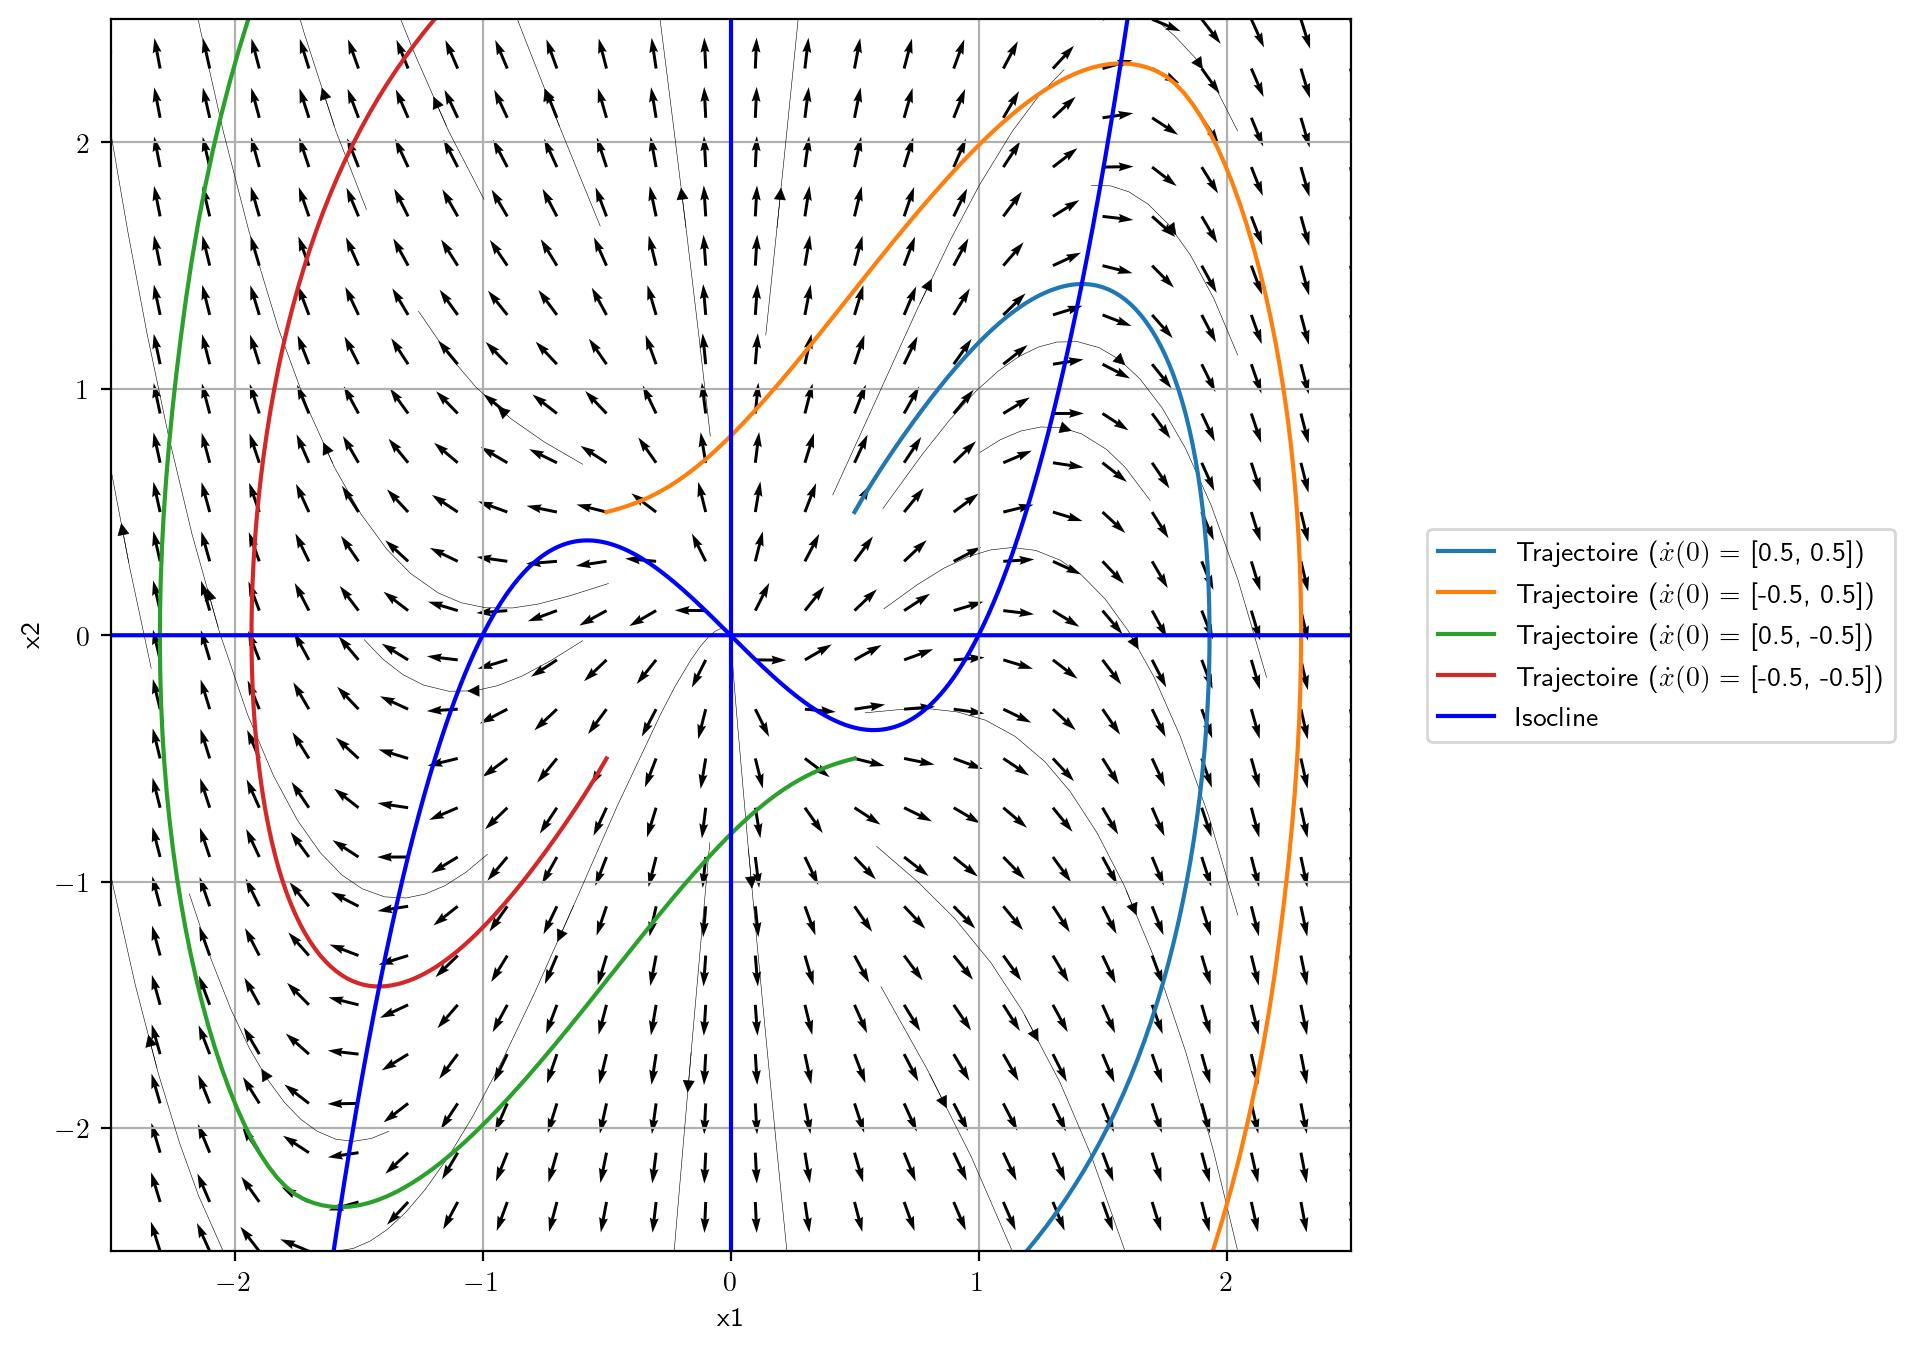
\includegraphics[width=\textwidth]{images/pdp_exercice_3_2.jpg}
                \caption{Solution numérique de l'exercice 2}
                \label{fig:pdp_exercice_3_2}
            \end{figure}

        \subsection{Exercice 3}
            \begin{exercise}{Exercice 3}
                \begin{equation}
                    \begin{cases}
                        \dot{x}_1 = 0.2 x_1 - 0.08 x_1 x_2 \\
                        \dot{x}_2 = 0.1 x_1 x_2 - 0.2 x_2
                    \end{cases}
                \end{equation}
            \end{exercise}
            La solution numérique est donnée à titre indicatif dans la figure \ref{fig:pdp_exercice_3_3}.
            \begin{figure}[ht!]
                \centering
                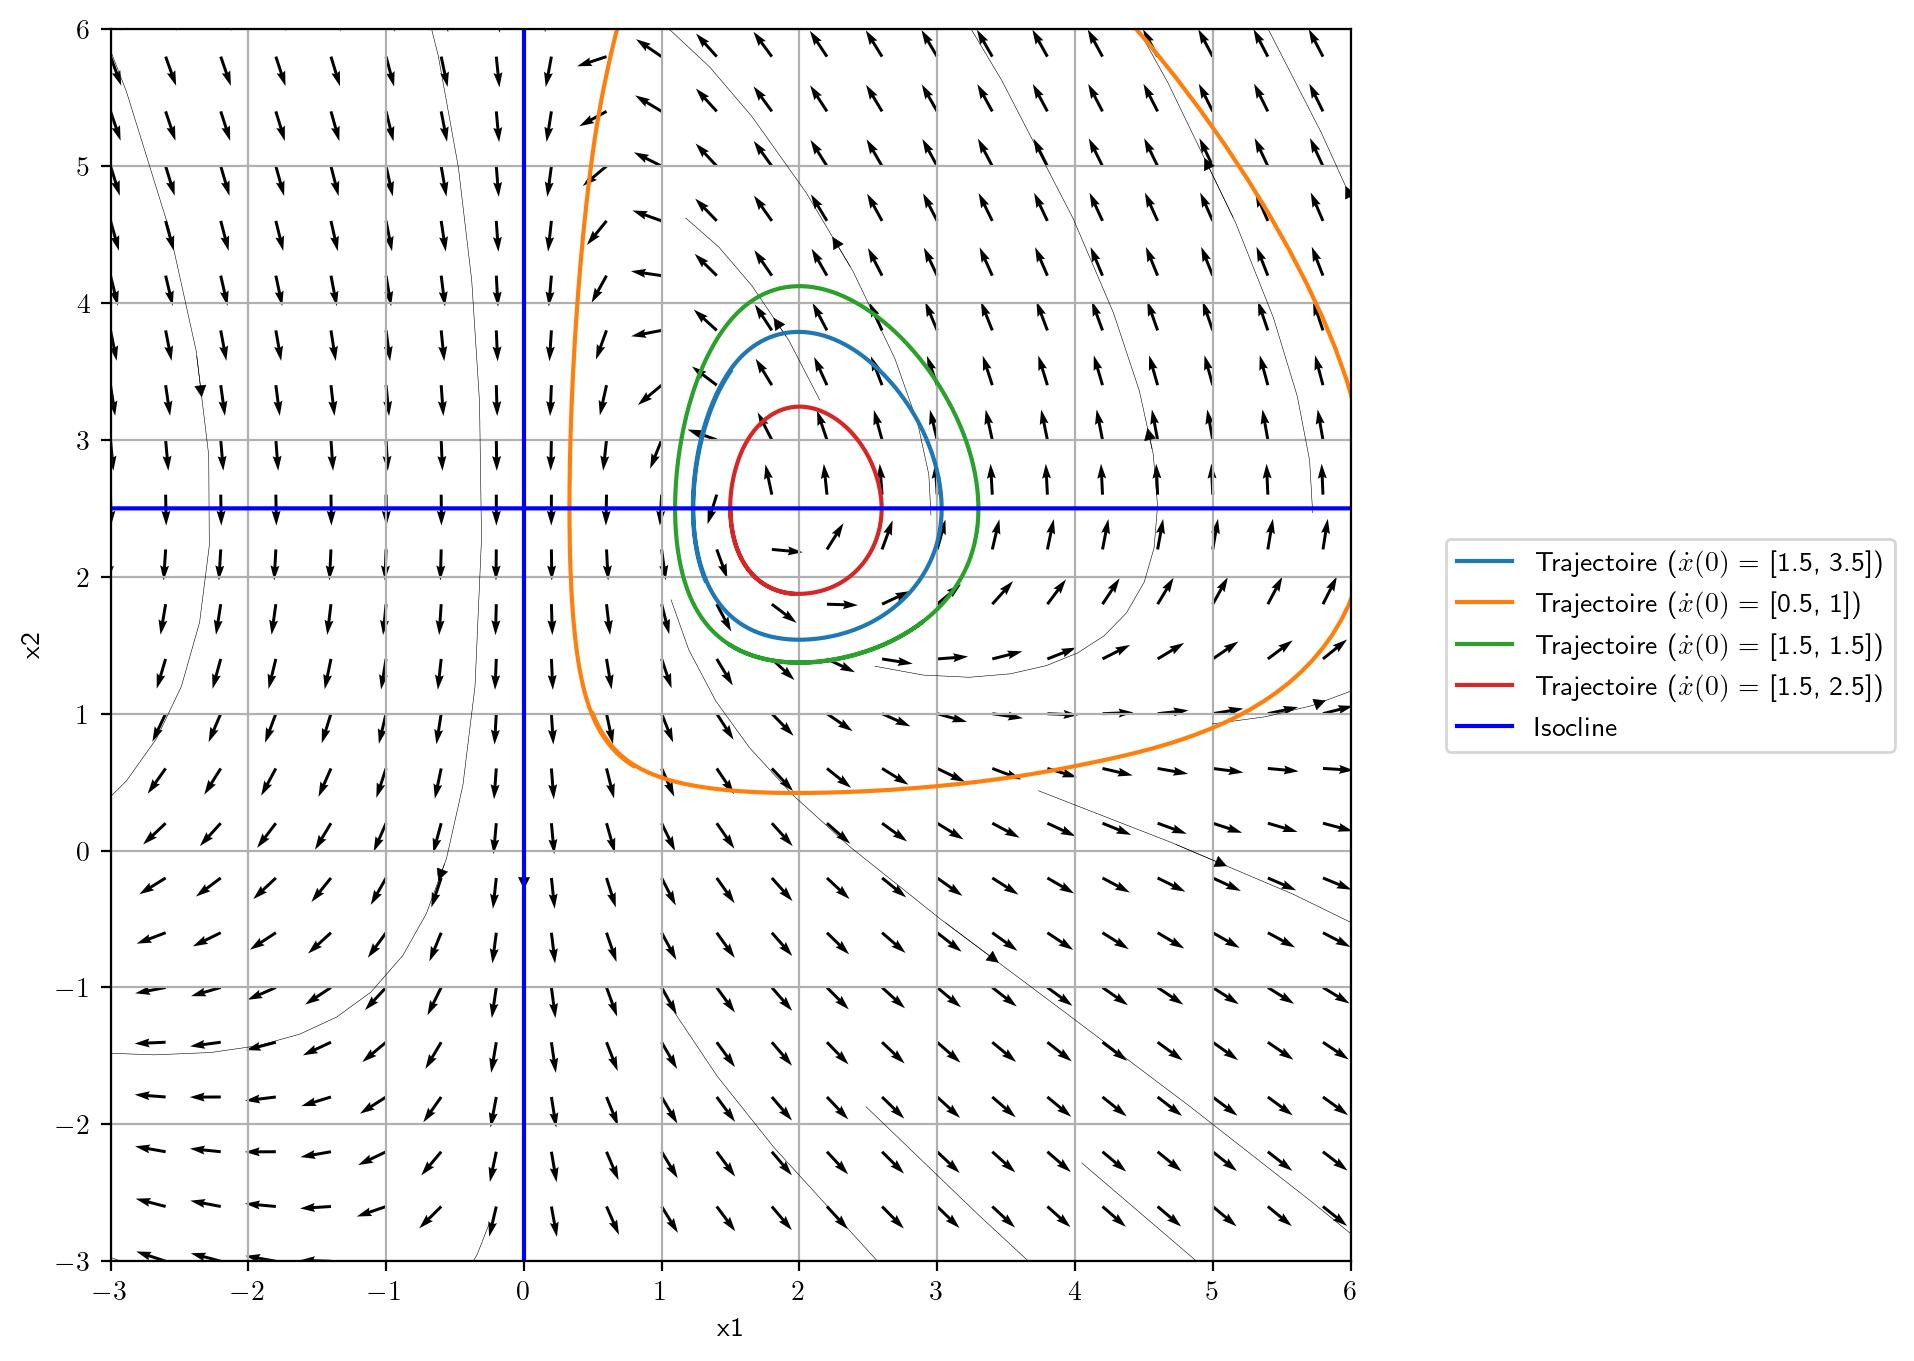
\includegraphics[width=\textwidth]{images/pdp_exercice_3_3.jpg}
                \caption{Solution numérique de l'exercice 3}
                \label{fig:pdp_exercice_3_3}
            \end{figure}
